\documentclass[0-protokol.tex]{subfiles}
\begin{document}

Výkon střídavého proudu závisí na fázovém posunu napětí vůči proudu $\varphi$ vztahem
\begin{equation} \label{eq:vykon}
P = UI \cos \varphi,
\end{equation}
kde $U$ a $I$ jsou efektivní hodnoty napětí a proudu.

Pomocí komplexního formalismu řešení střídavých obvodů je možné odvodit vztahy pro absolutní hodnotu komplexní impedance $Z = \frac{U}{I}$ a fázový posun napětí vůči proudu $\varphi$ sériového RL obvodu
\begin{equation}
Z = \sqrt{R^2 + \omega^2 L^2},
\end{equation}
\begin{equation}
\varphi = \arctan \frac{\omega L}{R}
\end{equation}
a paralelního RL obvodu
\begin{equation}
\frac{1}{Z} = \sqrt{\frac{1}{R^2} + \frac{1}{\omega^2 L^2}},
\end{equation}
\begin{equation}
\varphi = \arctan \left(\frac{R}{\omega L} \right).
\end{equation}

Z těchto vztahů pak plynou rovnice pro odpor a indukčnost prvků
\begin{equation} \label{eq:R_s}
R_s = \frac{U}{I}\frac{1}{\sqrt{1 + \tan^2 \varphi}},
\end{equation}
\begin{equation} \label{eq:L_s}
L_s = \frac{1}{\omega}\frac{U}{I}\sqrt{\frac{\tan^2 \varphi}{1 + \tan^2 \varphi}}
\end{equation}
v sériovém a
\begin{equation} \label{eq:R_p}
R_p = \frac{U}{I}\sqrt{1 + \tan^2 \varphi},
\end{equation}
\begin{equation} \label{eq:L_p}
L_p = \frac{1}{\omega}\frac{U}{I}\sqrt{\frac{1 + \tan^2 \varphi}{\tan^2 \varphi}}
\end{equation}
v paralelním zapojení. V těchto vztazích je $\omega = 2 \pi f$ úhlová frekvence střídavých veličin.

Pro měření účiníku bylo použito zapojení z obrázku \ref{fig:zap}.

\begin{figure}[H]
\centering
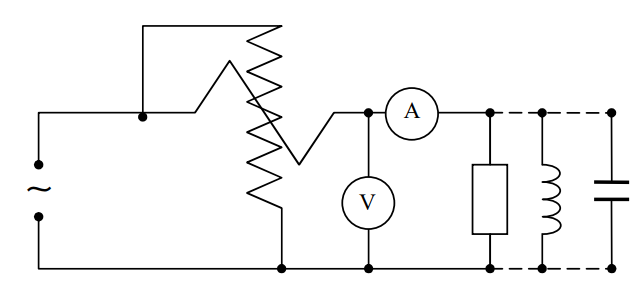
\includegraphics[scale=0.5]{zap}
\caption{Zapojení pro měření účiníku}
\label{fig:zap}
\end{figure}
\end{document}
